% !TEX root = main.tex

% TODO:
% REMARK:

\section{Data and Simulation samples}
\label{sec:DataAndMC}

	\subsection{Data sample}
	\label{ssec:DataAndMC_Data}

		In the analysis, the data is collected from CMS detector in 2016. CMS data are aggregated into $\textbf{lumisection}$ each taking corresponds to a 23 seconds of data taking\cite{Borisyak_2017}. Also, the detector is turned on and taking data in a non-stop period which is called $\textbf{run}$. A run stores the events which are taken under the same condition of detectors and plenty of lumisections are under each run. The used lumisection in this analysis are in good condition. The $\textbf{era}$ represent a series of date collection as long as a significant change to the detector configuration. There are some misbehaving of subdetectors' components on a per-lumisection basis. There are joint efforts of all subdetector's experts to remove these data, called $\textbf{lumimask}$. The good data lumisection are selected by $\emph{golden json file}$ in the implementation aspect.The datasets we used in this analysis are shown below:

		\begin{center}
		\setlength{\tabcolsep}{12pt}
		\begin{longtable}{ | c | c | }
		\caption{2016 dataset (SingleMuon)} \\
		\hline
		dataset & $L$ [$fb^{-1}$]\\
		\hline
		/SingleMuon/Run2016B-17Jul2018 ver2-v1/MINIAOD & 5.75 \\
		/SingleMuon/Run2016C-17Jul2018-v1/MINIAOD & 2.57 \\
		/SingleMuon/Run2016D-17Jul2018-v1/MINIAOD & 4.24 \\
		/SingleMuon/Run2016E-17Jul2018-v1/MINIAOD & 4.03 \\
		/SingleMuon/Run2016F-17Jul2018-v1/MINIAOD & 3.10 \\
		/SingleMuon/Run2016G-17Jul2018-v1/MINIAOD & 7.58 \\
		/SingleMuon/Run2016H-17Jul2018-v1/MINIAOD & 8.65 \\
		\hline
		\end{longtable}
		\label{DataAndMC:tb:dataset_mu}
		\end{center}

		\begin{center}
		\setlength{\tabcolsep}{12pt}
		\begin{longtable}{ | c | c | }
		\caption{2016 dataset (SingleElectron)} \\
		\hline
		dataset & $L$ [$fb^{-1}$]\\
		\hline
		/SingleElectron/Run2016B-17Jul2018 ver2-v1/MINIAOD & 5.75 \\
		/SingleElectron/Run2016C-17Jul2018-v1/MINIAOD & 2.57 \\
		/SingleElectron/Run2016D-17Jul2018-v1/MINIAOD & 4.24 \\
		/SingleElectron/Run2016E-17Jul2018-v1/MINIAOD & 4.03 \\
		/SingleElectron/Run2016F-17Jul2018-v1/MINIAOD & 3.10 \\
		/SingleElectron/Run2016G-17Jul2018-v1/MINIAOD & 7.58 \\
		/SingleElectron/Run2016H-17Jul2018-v1/MINIAOD & 8.65 \\
		\hline
		\end{longtable}
		\label{DataAndMC:tb:dataset_el}
		\end{center}

		We can find that there are two different type of datasets are used for the electron and muon channels in the analysis. It is about the dataset pass the single lepton HLTs. That is to say, the dataset named $\emph{SingleMuon}$ includes the events which have at least one muon as its name, and so do $\emph{SingleElectron}$ datasets. The adoption of HLT first on dataset could make convinience and simplification of starting analysis computing. Obviously, the SingleMuon and SingleElectron dataset would be appropriate to the signal which is semi-leptonic $t\bar{t}$. The integrated luminosity of both SingleElectron and SingleMuon are $35.9 fb^{-1}$.

	\subsection{Simulated sample}
	\label{ssec:DataAndMC_MC}

		The necessary simulated samples are considered varying when being applied on changing analysis, that is, the different physical process are needed in analysises. The simulated samples are just like the real data being able to be detected by the detectors, but we know which physical process are these events from. To generate these process' simulated samples, the $\textbf{Monte Carlo(MC)}$ method is used. The Monte Carlo method, whose generated algorithm is related to random number generator, is frequently used in some fields with probabilistic issues. In this analysis, simulation sample and MC sample are the same thing in the following contents.

		The physical processes are first generated in parton level by particular generator(ex.Madgraph\cite{Alwall:2011uj}, powheg\cite{Frixione:2007nu}) with $\textbf{parton distribution function}$, and being to be the peoduction in matix elements level. The parton showering from matrix elements level are nextly simulated by some tool(ex.Pythia\cite{Sjostrand:2014zea}). Then the final decay particles are from GEANT4-based\cite{Agostinelli:2002hh} simulation. The GEANT4 simulator may produce final physical objects from parton level's events. It can even imitate the representation of electronics, interaction with geometry structure of detectors and detector's resolution, etc. The simulation datasets are the results of GEANT4 with passing L1T(level 1 trigger, section.\ref{ssec:PhysObj_trg}). Eventually, after passing HLT(high level trigger, section.\ref{ssec:PhysObj_trg}), the events with physical objects are reconstructed. The illustration diagram of generating is shown as Fig.ref*****

		The signal simulated events in this analysis -- $t\bar{t}$'s semi-leptonic decay process is expected to be dominant after manipulating on all simulated samples. Rather than the next-to-leading order(NLO) QCD precision, the next-to-NLO(NNLO) parton distribution function\cite{Ball:2017nwa} is used to signal $t\bar{b}$ semi-leptonic sample. The default value of invariant mass of top($m_{t}$) is set to 172.5GeV in all simulations. All simulation's generating information are shown below(\ref{DataMC:tb:process}) including process name, corresponding cross section, k-factor, generatted events number and used generator. The k-factor is the factor to compensate the LO(leading order term) sample's high order terms' cross section. The corresponding files name is also shown below(\ref{DataMC:tb:filename}.

		%%% table of the MC sample's Xsec and generated events number and generator -> weight to luminosity

		\begin{center}
		\begin{longtable}{ | c c c c c | }
		\caption{Informations of simulated samples used in this analysis} \\
		\hline
		Process sample & Cross Section[pb] & k-factor & Events No. & Generator \\ 
		\hline
		$t$$\bar{t}\rightarrow b \bar{b}jjl\nu$ & $365.34$(NNLO) & $1$ & $106736180$ & powheg \\
		\hline
		$Z / \gamma * \rightarrow l^+ l^-$, $H_{T}$ $\in [70,100)$GeV & $169.9$(LO) & $1.23$ & $9388811$ & Madgraph \\
		$Z / \gamma * \rightarrow l^+ l^-$, $H_{T}$ $\in [100,200)$GeV & $147.4$(LO) & $1.23$ & $8265899$ & Madgraph \\
		$Z / \gamma * \rightarrow l^+ l^-$, $H_{T}$ $\in [200,400)$GeV & $41.0$(LO) & $1.23$ & $8646942$ & Madgraph \\
		$Z / \gamma * \rightarrow l^+ l^-$, $H_{T}$ $\in [400,600)$GeV & $5.7$(LO) & $1.23$ & $8527128$ & Madgraph \\
		$Z / \gamma * \rightarrow l^+ l^-$, $H_{T}$ $\in [600,800)$GeV & $1.4$(LO) & $1.23$ & $8533247$ & Madgraph \\
		$Z / \gamma * \rightarrow l^+ l^-$, $H_{T}$ $\in [800,1200)$GeV & $6.3 \times 10^{-1}$(LO) & $1.23$ & $2673006$ & Madgraph \\
		$Z / \gamma * \rightarrow l^+ l^-$, $H_{T}$ $\in [1200,2500)$GeV & $1.5 \times 10^{-1}$(LO) & $1.23$ & $596079$ & Madgraph \\
		$Z / \gamma * \rightarrow l^+ l^-$, $H_{T}$ $\in [2500, \infty )$GeV & $3.6 \times 10^{-3}$(LO) & $1.23$ & $399492$ & Madgraph \\
		\hline
		W+jets$\rightarrow l \nu$, $H_{T}$ $\in [100,200)$GeV & $1345.7$(LO) & $1.21$ & $38593839$ & Madgraph \\
		W+jets$\rightarrow l \nu$, $H_{T}$ $\in [200,400)$GeV & $359.7$(LO) & $1.21$ & $19914590$ & Madgraph \\
		W+jets$\rightarrow l \nu$, $H_{T}$ $\in [400,600)$GeV & $48.9$(LO) & $1.21$ & $5796237$ & Madgraph \\
		W+jets$\rightarrow l \nu$, $H_{T}$ $\in [600,800)$GeV & $12.1$(LO) & $1.21$ & $14908339$ & Madgraph \\
		W+jets$\rightarrow l \nu$, $H_{T}$ $\in [800,1200)$GeV & $5.5$(LO) & $1.21$ & $6286023$ & Madgraph \\
		W+jets$\rightarrow l \nu$, $H_{T}$ $\in [1200,2500)$GeV & $1.3$(LO) & $1.21$ & $6677967$ & Madgraph \\
		W+jets$\rightarrow l \nu$, $H_{T}$ $\in [2500,\infty)$GeV & $3.2 \times 10^{-2}$(LO) & $1.21$ & $2384260$ & Madgraph \\
		\hline
		$WW$ & $118.7$(NLO) & $1$ & $6988168$ & Madgraph \\
		$WZ$ & $47.1$(NLO) & $1$ & $2997571$ & Madgraph \\
		$ZZ$ & $16.5$(NLO) & $1$ & $998034$ & Madgraph \\
		\hline
		SingleTop s-channel($t,\bar{t}$) & $3.36$(NLO) & $1$ & $6137801$ & powheg \\
		SingleTop t-channel($t$) & $136.02$(NLO) & $1$ & $67105876$ & powheg \\
		SingleTop t-channel($\bar{t}$) & $80.95$(NLO) & $1$ & $17780700$ & powheg \\
		SingleTop tW-channel($t$) & $35.6$(NLO) & $1$ & $4945734$ & powheg \\
		SingleTop tW-channel($\bar{t}$) & $35.6$(NLO) & $1$ & $4942374$ & powheg \\
		\hline
		QCD, $H_{T}$ $\in [100,200)$GeV & $2.799 \times 10^{7}$(LO) & $1$ & $82293477$ & Madgraph \\
		QCD, $H_{T}$ $\in [200,300)$GeV & $1.712 \times 10^{6}$(LO) & $1$ & $38857977$ & Madgraph \\
		QCD, $H_{T}$ $\in [300,500)$GeV & $3.477 \times 10^{5}$(LO) & $1$ & $37516961$ & Madgraph \\
		QCD, $H_{T}$ $\in [500,700)$GeV & $3.21 \times 10^{4}$(LO) & $1$ & $44061688$ & Madgraph \\
		QCD, $H_{T}$ $\in [700,1000)$GeV & $6831$(LO) & $1$ & $21604533$ & Madgraph \\
		QCD, $H_{T}$ $\in [1000,1500)$GeV & $1207$(LO) & $1$ & $10286971$ & Madgraph \\
		QCD, $H_{T}$ $\in [1500,2000)$GeV & $119.9$(LO) & $1$ & $7868538$ & Madgraph \\
		QCD, $H_{T}$ $\in [2000,\infty)$GeV & $25.2$(LO) & $1$ & $4027896$ & Madgraph \\
		\hline
		\label{DataMC:tb:process}
		\end{longtable}
		\end{center}

		\begin{center}
		\begin{longtable}{ | c | }
		\caption{Corresponding file's name with process in the same arrangement in Table.\ref{DataMC:tb:process}} \\
		\hline
		File name \\ 
		\hline
		TTToSemiLeptonic\_TuneCP5\_PSweights\_13TeV-powheg-pythia8 \\
		\hline
		DYJetsToLL\_M-50\_HT-70to100\_TuneCUETP8M1\_13TeV-madgraphMLM-pythia8 \\
		DYJetsToLL\_M-50\_HT-100to200\_TuneCUETP8M1\_13TeV-madgraphMLM-pythia8 \\
		DYJetsToLL\_M-50\_HT-200to400\_TuneCUETP8M1\_13TeV-madgraphMLM-pythia8 \\
		DYJetsToLL\_M-50\_HT-400to600\_TuneCUETP8M1\_13TeV-madgraphMLM-pythia8 \\
		DYJetsToLL\_M-50\_HT-600to800\_TuneCUETP8M1\_13TeV-madgraphMLM-pythia8 \\
		DYJetsToLL\_M-50\_HT-800to1200\_TuneCUETP8M1\_13TeV-madgraphMLM-pythia8 \\
		DYJetsToLL\_M-50\_HT-1200to2500\_TuneCUETP8M1\_13TeV-madgraphMLM-pythia8 \\
		DYJetsToLL\_M-50\_HT-2500toInf\_TuneCUETP8M1\_13TeV-madgraphMLM-pythia8 \\
		\hline
		WJetsToLNu\_HT-100To200\_TuneCUETP8M1\_13TeV-madgraphMLM-pythia8 \\
		WJetsToLNu\_HT-200To400\_TuneCUETP8M1\_13TeV-madgraphMLM-pythia8 \\
		WJetsToLNu\_HT-400To600\_TuneCUETP8M1\_13TeV-madgraphMLM-pythia8 \\
		WJetsToLNu\_HT-600To800\_TuneCUETP8M1\_13TeV-madgraphMLM-pythia8 \\
		WJetsToLNu\_HT-800To1200\_TuneCUETP8M1\_13TeV-madgraphMLM-pythia8 \\
		WJetsToLNu\_HT-1200To2500\_TuneCUETP8M1\_13TeV-madgraphMLM-pythia8 \\
		WJetsToLNu\_HT-2500ToInf\_TuneCUETP8M1\_13TeV-madgraphMLM-pythia8 \\
		\hline
		WW\_TuneCUETP8M1\_13TeV-pythia8 \\
		WZ\_TuneCUETP8M1\_13TeV-pythia8 \\
		ZZ\_TuneCUETP8M1\_13TeV-pythia8 \\
		\hline
		ST\_s-channel\_4f\_leptonDecays\_TuneCP5\_PSweights\_13TeV-amcatnlo-pythia8 \\
		ST\_t-channel\_top\_4f\_inclusiveDecays\_13TeV-powhegV2-madspin-pythia8\_TuneCUETP8M1 \\
		ST\_t-channel\_antitop\_4f\_InclusiveDecays\_TuneCP5\_PSweights\_13TeV-powheg-pythia8 \\
		ST\_tW\_top\_5f\_inclusiveDecays\_TuneCP5\_PSweights\_13TeV-powheg-pythia8 \\
		ST\_tW\_antitop\_5f\_inclusiveDecays\_TuneCP5\_PSweights\_13TeV-powheg-pythia8 \\
		\hline
		QCD\_HT100to200\_TuneCUETP8M1\_13TeV-madgraphMLM-pythia8 \\
		QCD\_HT200to300\_TuneCUETP8M1\_13TeV-madgraphMLM-pythia8 \\
		QCD\_HT300to500\_TuneCUETP8M1\_13TeV-madgraphMLM-pythia8 \\
		QCD\_HT500to700\_TuneCUETP8M1\_13TeV-madgraphMLM-pythia8 \\
		QCD\_HT700to1000\_TuneCUETP8M1\_13TeV-madgraphMLM-pythia8 \\
		QCD\_HT1000to1500\_TuneCUETP8M1\_13TeV-madgraphMLM-pythia8 \\
		QCD\_HT1500to2000\_TuneCUETP8M1\_13TeV-madgraphMLM-pythia8 \\
		QCD\_HT2000toInf\_TuneCUETP8M1\_13TeV-madgraphMLM-pythia8 \\
		\hline
		\label{DataMC:tb:filename}
		\end{longtable}
		\end{center}



		Through highly developed simulation procedure, the simulated sample might be at the ideal stage as the real data. However, the simulated samples have their limitations and defects, so there are some coorrections on any events and physical objects(section.\ref{ssec:DataAndMC_corMC}), for example, the events weight is the common way to rescale the existance of any events, and it makes simulated sample's performance more similar to real data.

	\subsection{Correction on simulation sample}
	\label{ssec:DataAndMC_corMC}

		% pileup introduction is set on "vertex"
		\subsubsection{Pile-up Reweighing}
		\label{sssec:DataAndMC_PU}

			% https://twiki.cern.ch/twiki/bin/viewauth/CMS/PileupMCReweightingUtilities?fbclid=IwAR0SuZFQ5Um0IfZn1-CHXia6NPMYe2_7cz2OGXxhCYvNvfl_tTBke-w22l8

			As mention in section.\ref{ssec:PhysObj_pu}, pileup is the issue that bunch of vertices occuring at one collision. Although Monte Carlo sample may roughly cover the pileup interactions, the final distribution is also sensitive to the subtle content of primary vertex. Furthermore, the distribution of reconstructed vertices can be differently affected by the offline event selection cut and some high level trigger between real data and Monte Carlo sample. To fix the descrepancy between data and simulation, with any pileup number(number of primary vertices) bin, we compare the data and MC distribution and get the data/MC value bin by bin. The gotten scale factors under pileup number bins will be applied on the analyzed MC to correct the weight of each event.

		\subsubsection{Jet Energy correction, smearing and resolution}
		\label{sssec:DataAndMC_JE_CSR}

			The JEC and JER are mentioned in section.\ref{ssec:PhysObj_jet} previously.

		\subsubsection{Lepton efficiency Scale Factor}
		\label{sssec:DataAndMC_LepEffSF}

		With selection cut or quality pick-up on physics objects like leptons, there must be difference in the selection performance between data and MC. To correct the discrepancy, the often method is apply a scale factor on the $p_T$-$\eta$ space to correct the weight of this event. The scale factor S.F. is calculated from selection efficiency performance of known data and MC by Eq.\ref{eq:eff_SF}. 

		\begin{equation}
		S.F. = \frac{\epsilon_{data}(p_T,\eta)}{\epsilon_{MC}(p_T,\eta)}
		\label{eq:eff_SF}
		\end{equation}

		It is usually implemented by tag-and-probe method\cite{tagandprobe_twiki}. There are efficiency S.F. of muonISO, muonID, muonTrigger, ElectronReco, ElectronID, and ElectronTrigger necessary to be considered. The gotten scale factors under $p_T$-$\eta$ space are shown below:

		\begin{figure}[H]
			\centering
			    \subfigure[Muon ISO]{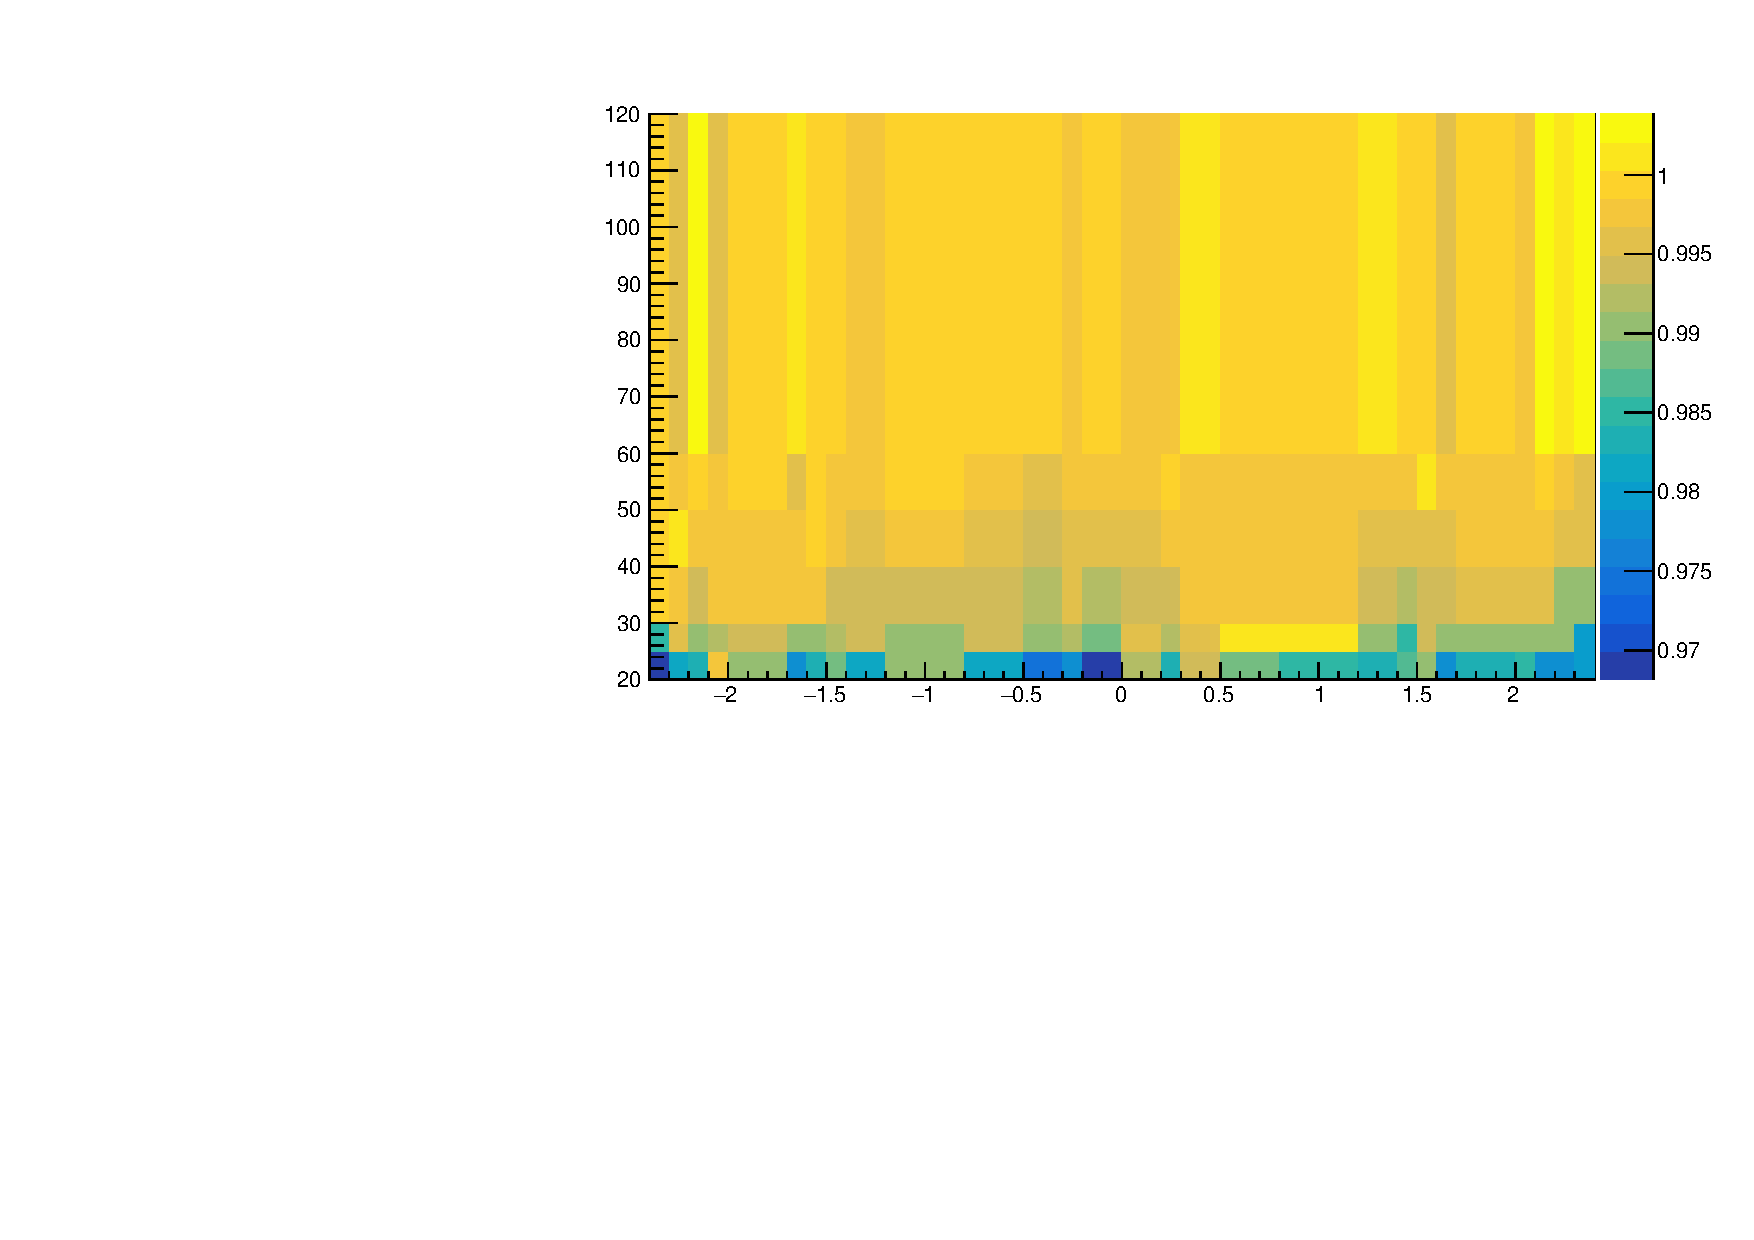
\includegraphics[width=0.32\textwidth]{Figures/DataMC/mu_ISO.pdf}}
			    \subfigure[Muon ID]{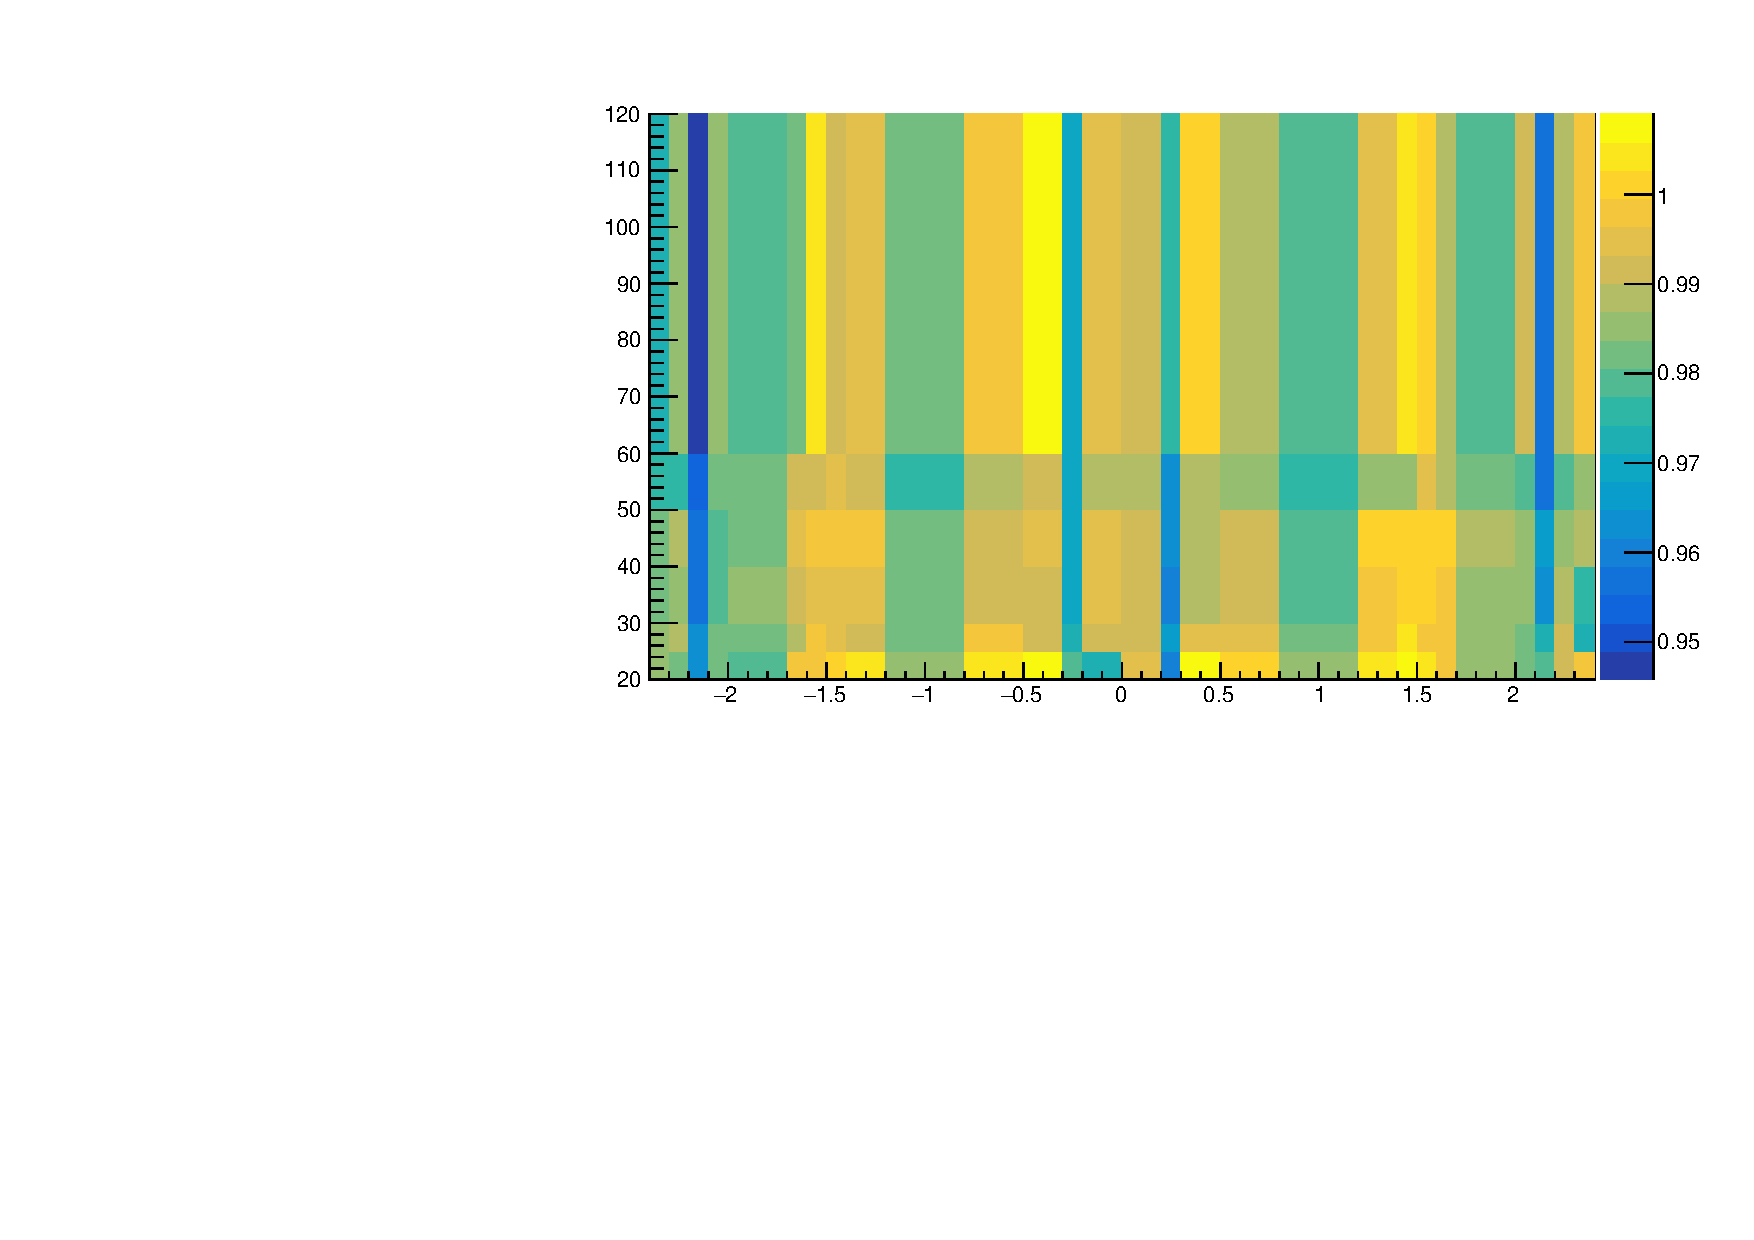
\includegraphics[width=0.32\textwidth]{Figures/DataMC/mu_ID.pdf}}
			    \subfigure[Muon High Level Trigger]{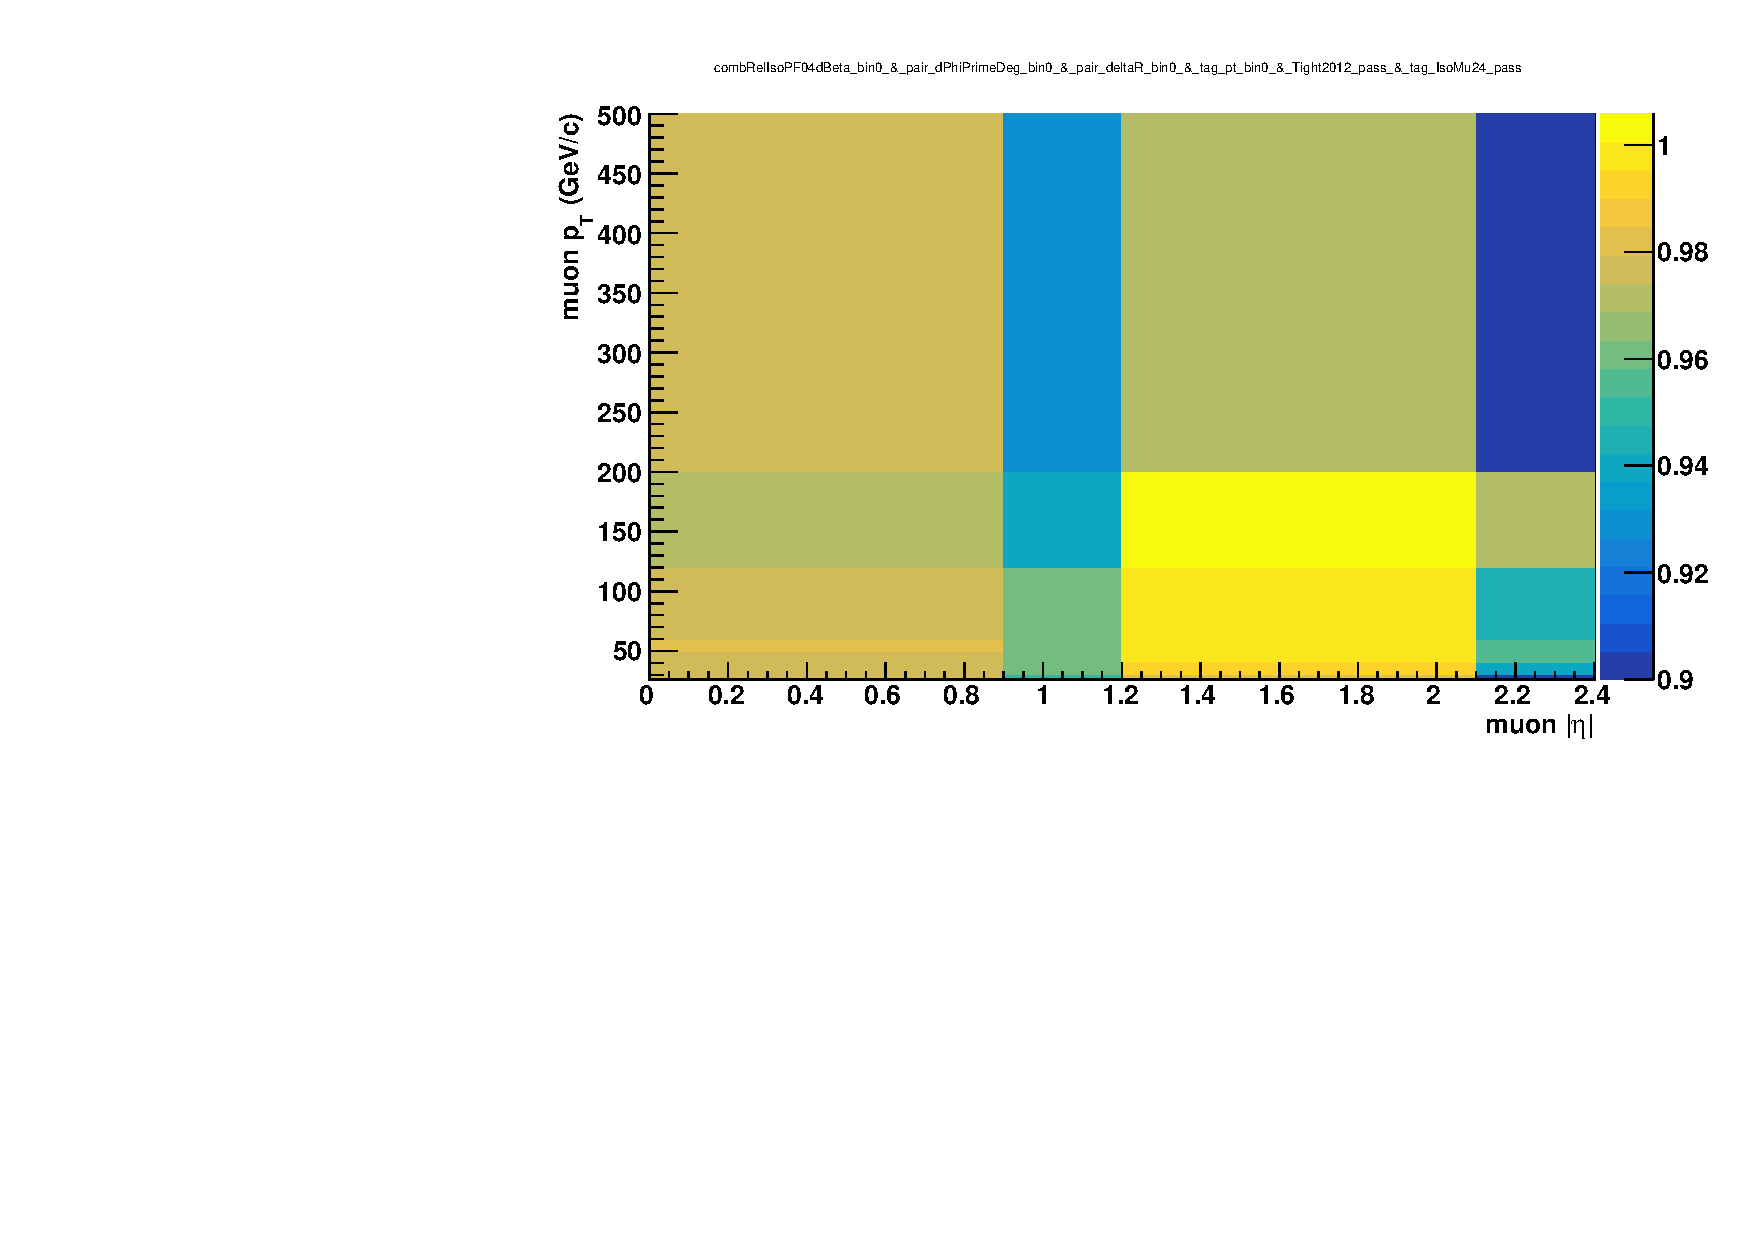
\includegraphics[width=0.32\textwidth]{Figures/DataMC/mu_Trg.pdf}}\\
			\end{figure}{}
			\FloatBarrier
			\begin{figure}[H]
			\centering
			    \subfigure[Electron Reco]{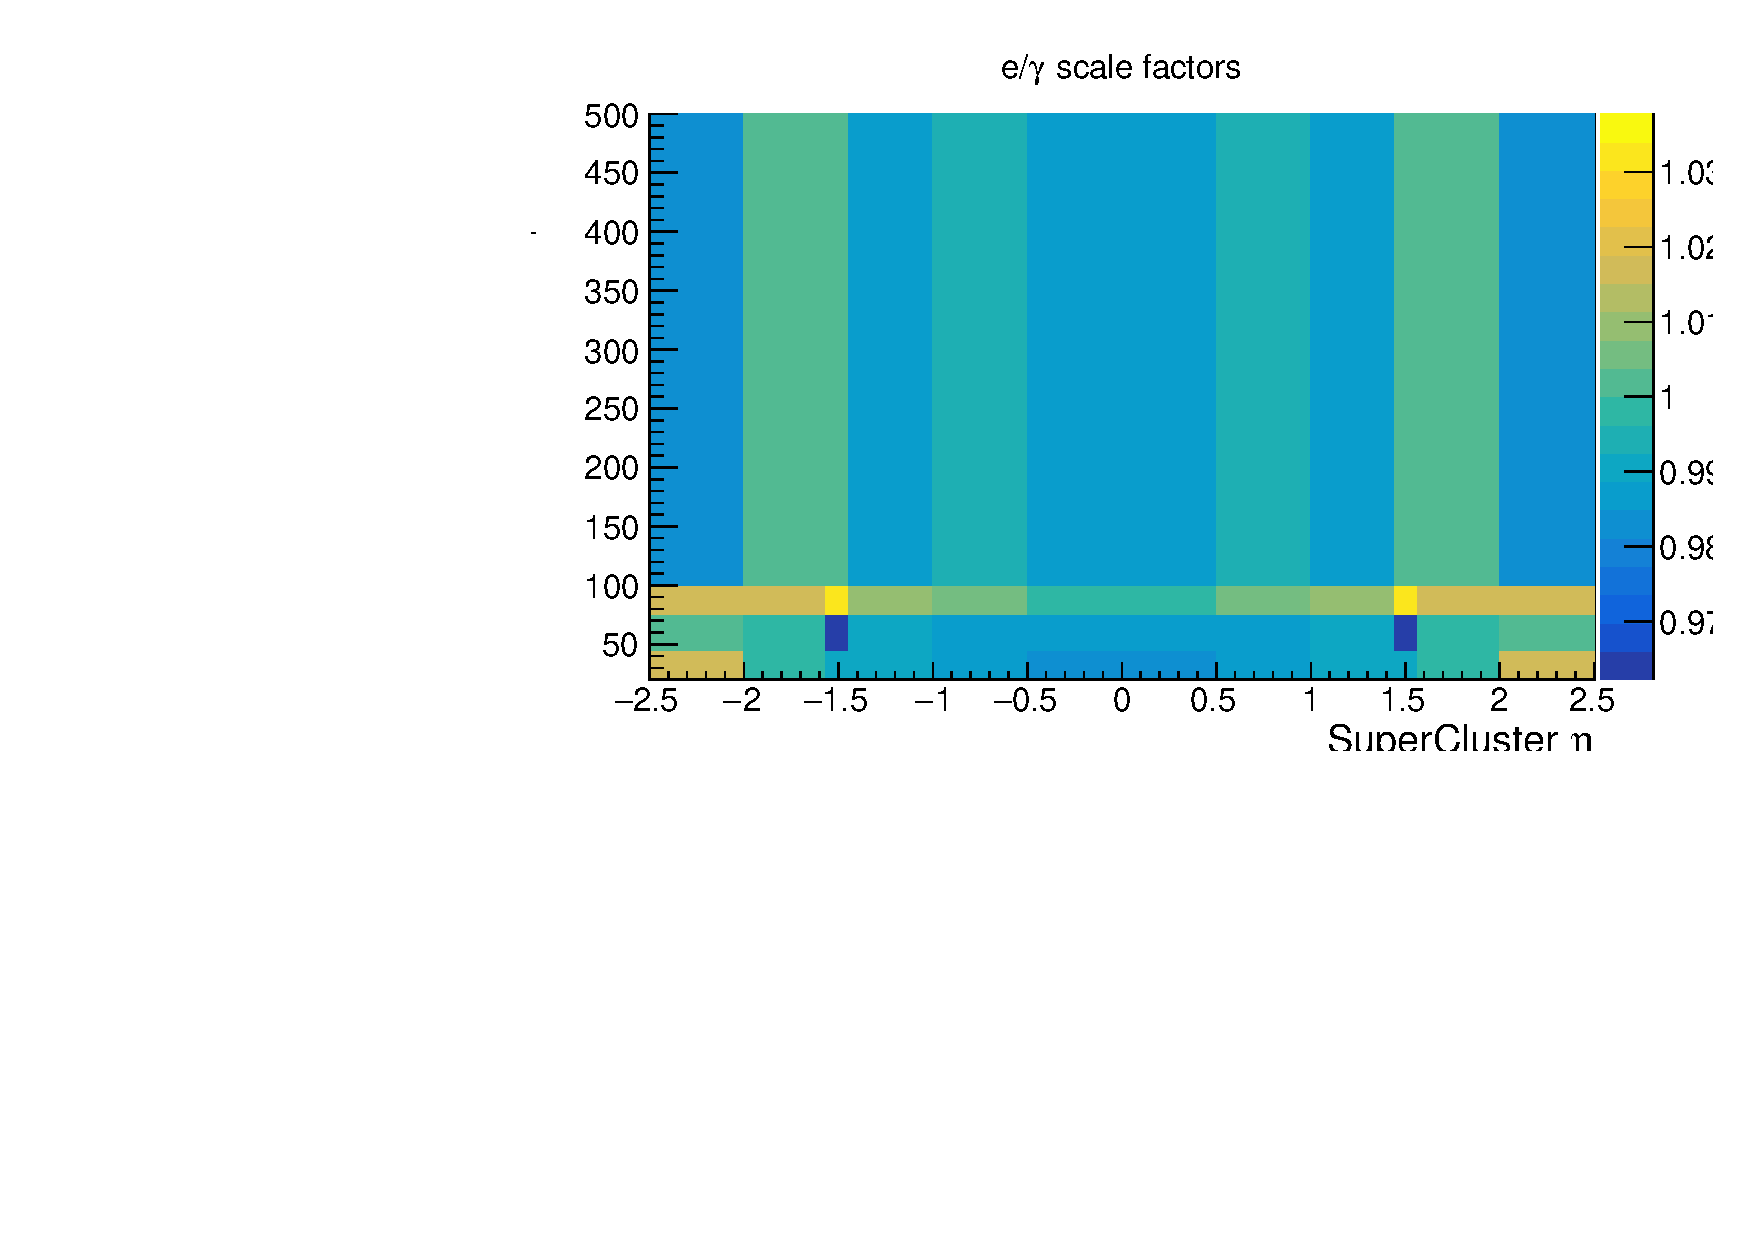
\includegraphics[width=0.32\textwidth]{Figures/DataMC/el_Reco.pdf}}
			    \subfigure[Electron ID]{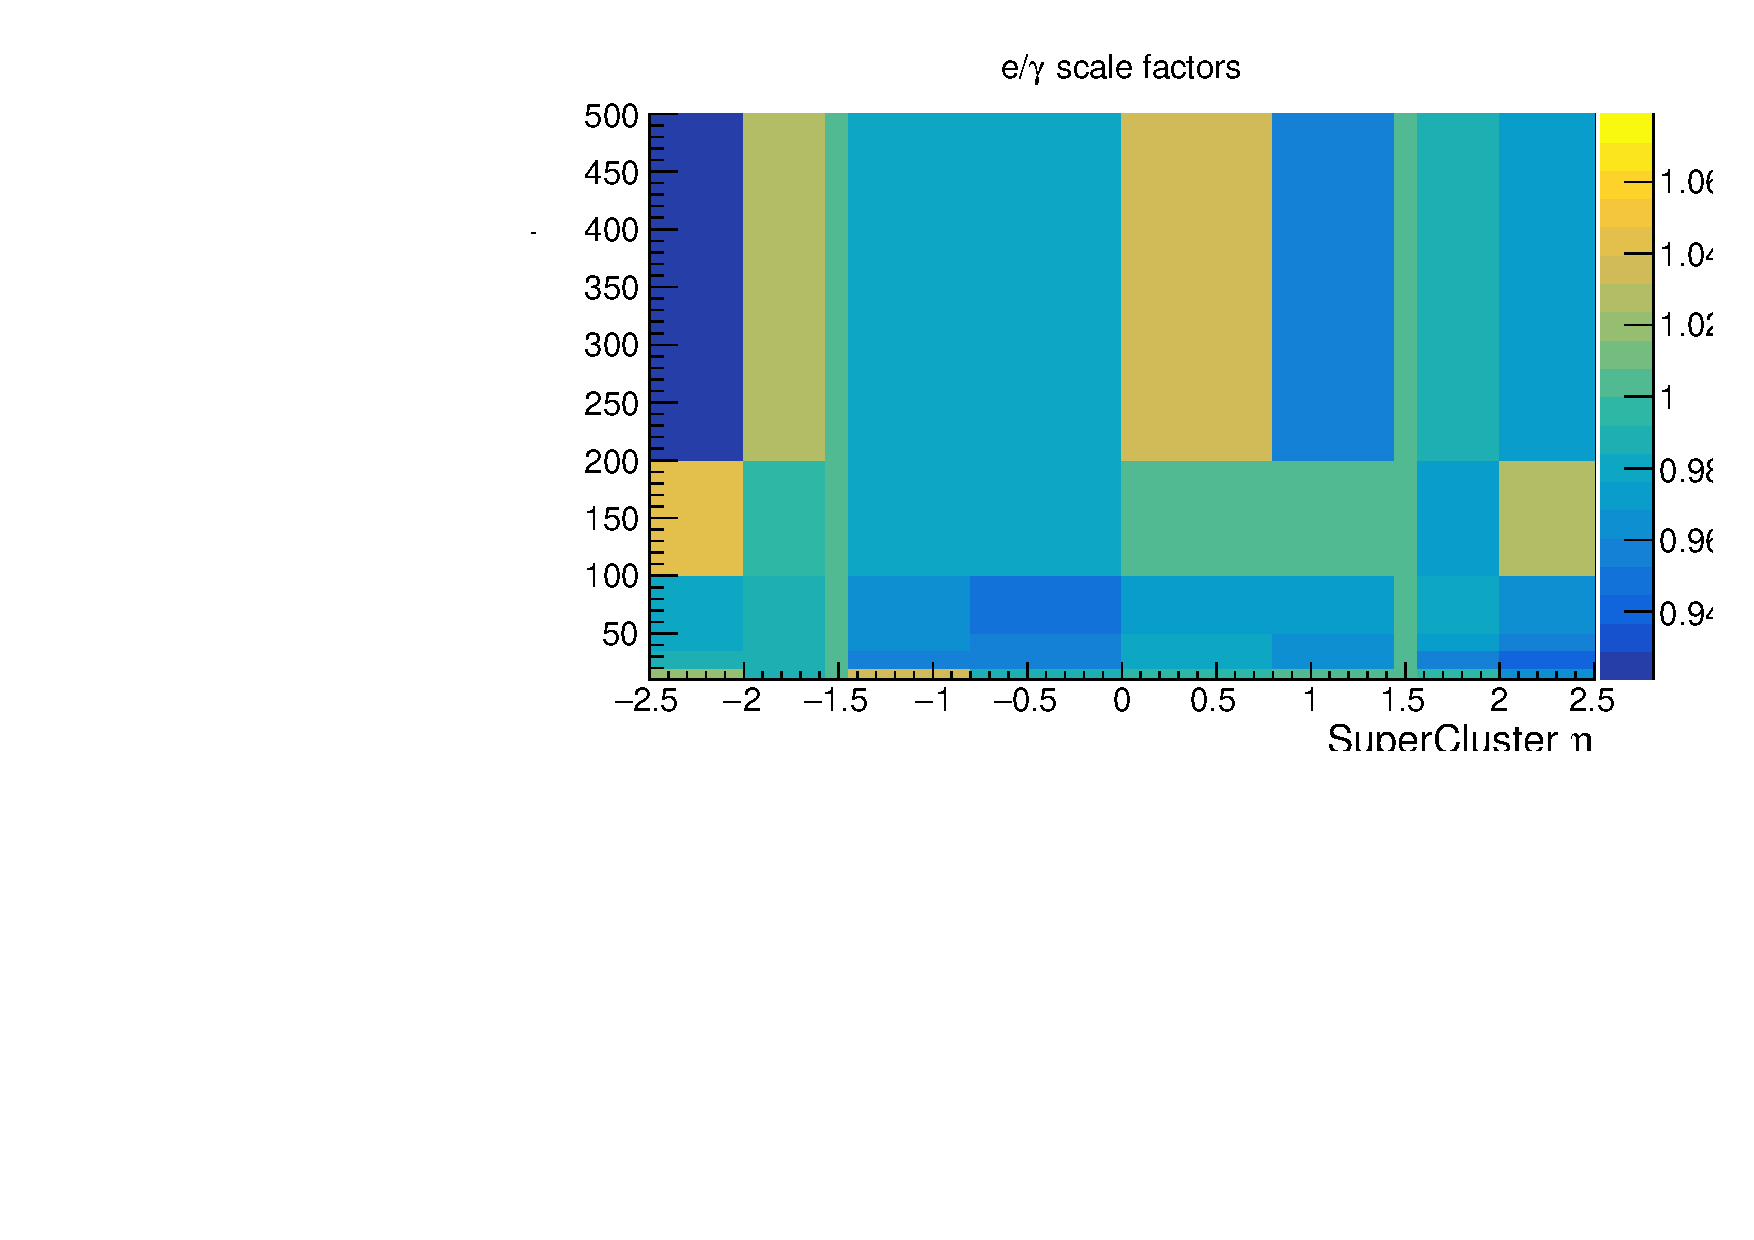
\includegraphics[width=0.32\textwidth]{Figures/DataMC/el_ID.pdf}}
			    \subfigure[Electron High Level Trigger]{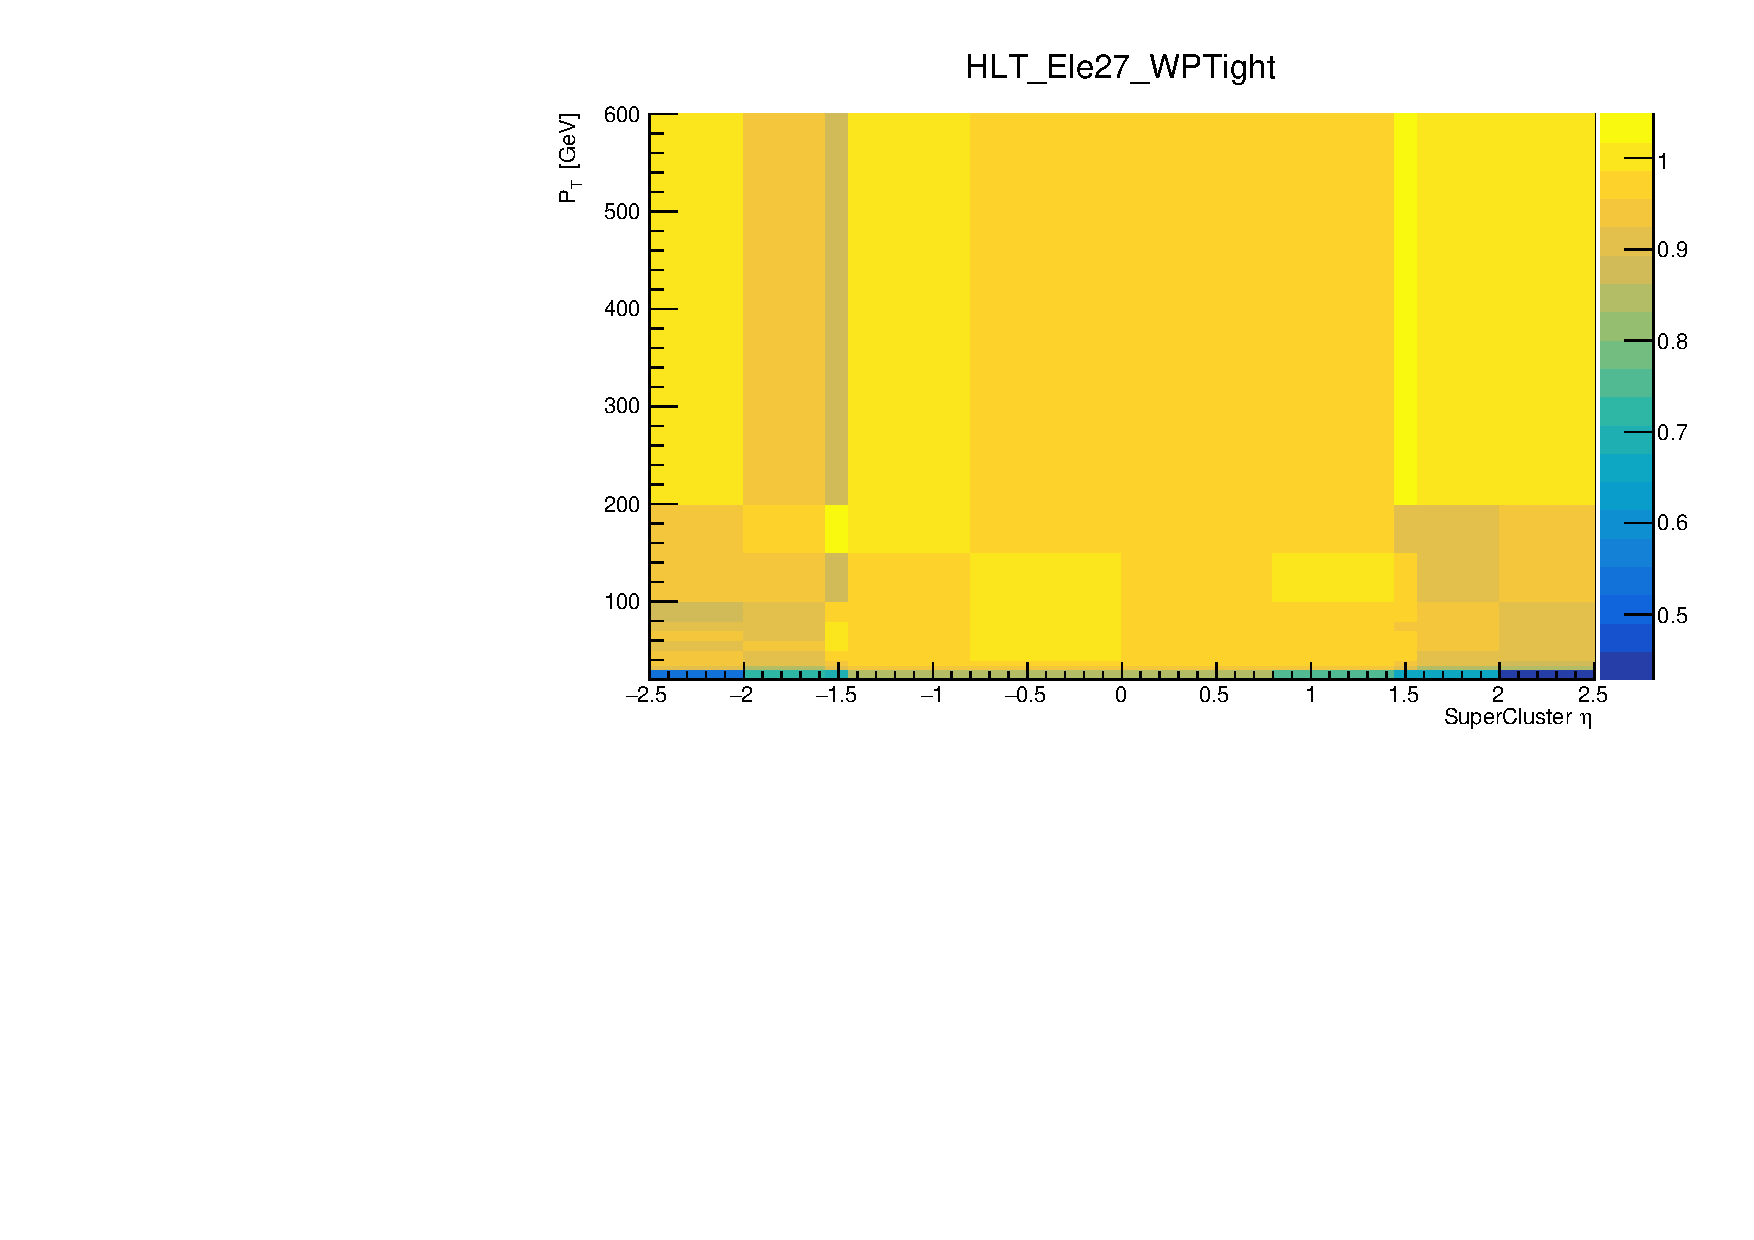
\includegraphics[width=0.32\textwidth]{Figures/DataMC/el_Trg.pdf}}\\
			   \caption{Lepton efficiency scale factor (x-axis:$\eta$, y-axis:$p_T$)}
			\label{DataMC:fig:lepsf}
			\end{figure}
			\FloatBarrier

		\subsubsection{b-tagging Reweighing}
		\label{sssec:DataAndMC_btagSF}

			The b-tagging reweight have to obtained by b-tagging scale factors and the b-tagging efficiency under b/c/light(udsg)-flavor identification.(The b-tagging efficiency means the ratio of jets which should pass b-tagging and really pass b-tagging) The b-tagging scale factor complies with the same concept as efficiency scale factor. Because of applying the selection which is deepCSV cut (DeepCSV Medium and DeepCSV Loose), data and MC have different performance on selection efficiency, then the S.F. of b-tagging is still got with Eq.\ref{eq:eff_SF} by BTV POG\cite{btvpog_twiki} with full RunII data. However, the reweight on each event is not just about scale factor. Since we apply the b-tagging tool on any jets which pass the jet-selection(Table.\ref{PhysObj:tb:sel_jet}), all the tagged jets and non-tagged jets should be considered to have influence about the b-tagging efficiency difference and to affect the event weight \cite{btagreweight_twiki}. The eventual formula of b-tagging event reweighting is derived by data correct tagged probability($P(data)$) divided by MC's($P(MC)$) (Eq.\ref{eq:btag_weight_1}). Both probabilities are calculated by Eq.\ref{eq:btag_weight_2} reasonabliy. 

			\begin{equation}
			weight = \frac{P(data)}{P(MC)}
			\label{eq:btag_weight_1}
			\end{equation}

			\begin{equation}
			\begin{split}
			P(MC) = \prod_{i=tagged} \epsilon_i(p_T,\eta) \prod_{j=non-tagged} (1-\epsilon_j(p_T,\eta)) \;\;\;\;\;\;\;\;\;\;\;\;\;\;\; \\
			P(data) = \prod_{i=tagged} SF(p_T,\eta) \cdot \epsilon_i(p_T,\eta) \prod_{j=non-tagged} (1- SF(p_T,\eta) \cdot \epsilon_j(p_T,\eta))
			\label{eq:btag_weight_2}
			\end{split}
			\end{equation}

			As mentioned previously, the S.F. are obtained, and b-tagging efficiency of three types of flavor jets are gotten by hand with simulated $t\bar{t}$ sample (Fig.\ref{DataMC:fig:tt_eff_btag}). Also, the b-tagging efficiency of three flavor jets are obviously different and they are calculated on the $p_T$-$\eta$ space.

			\begin{figure}[H]
			\centering
			    \subfigure[b]{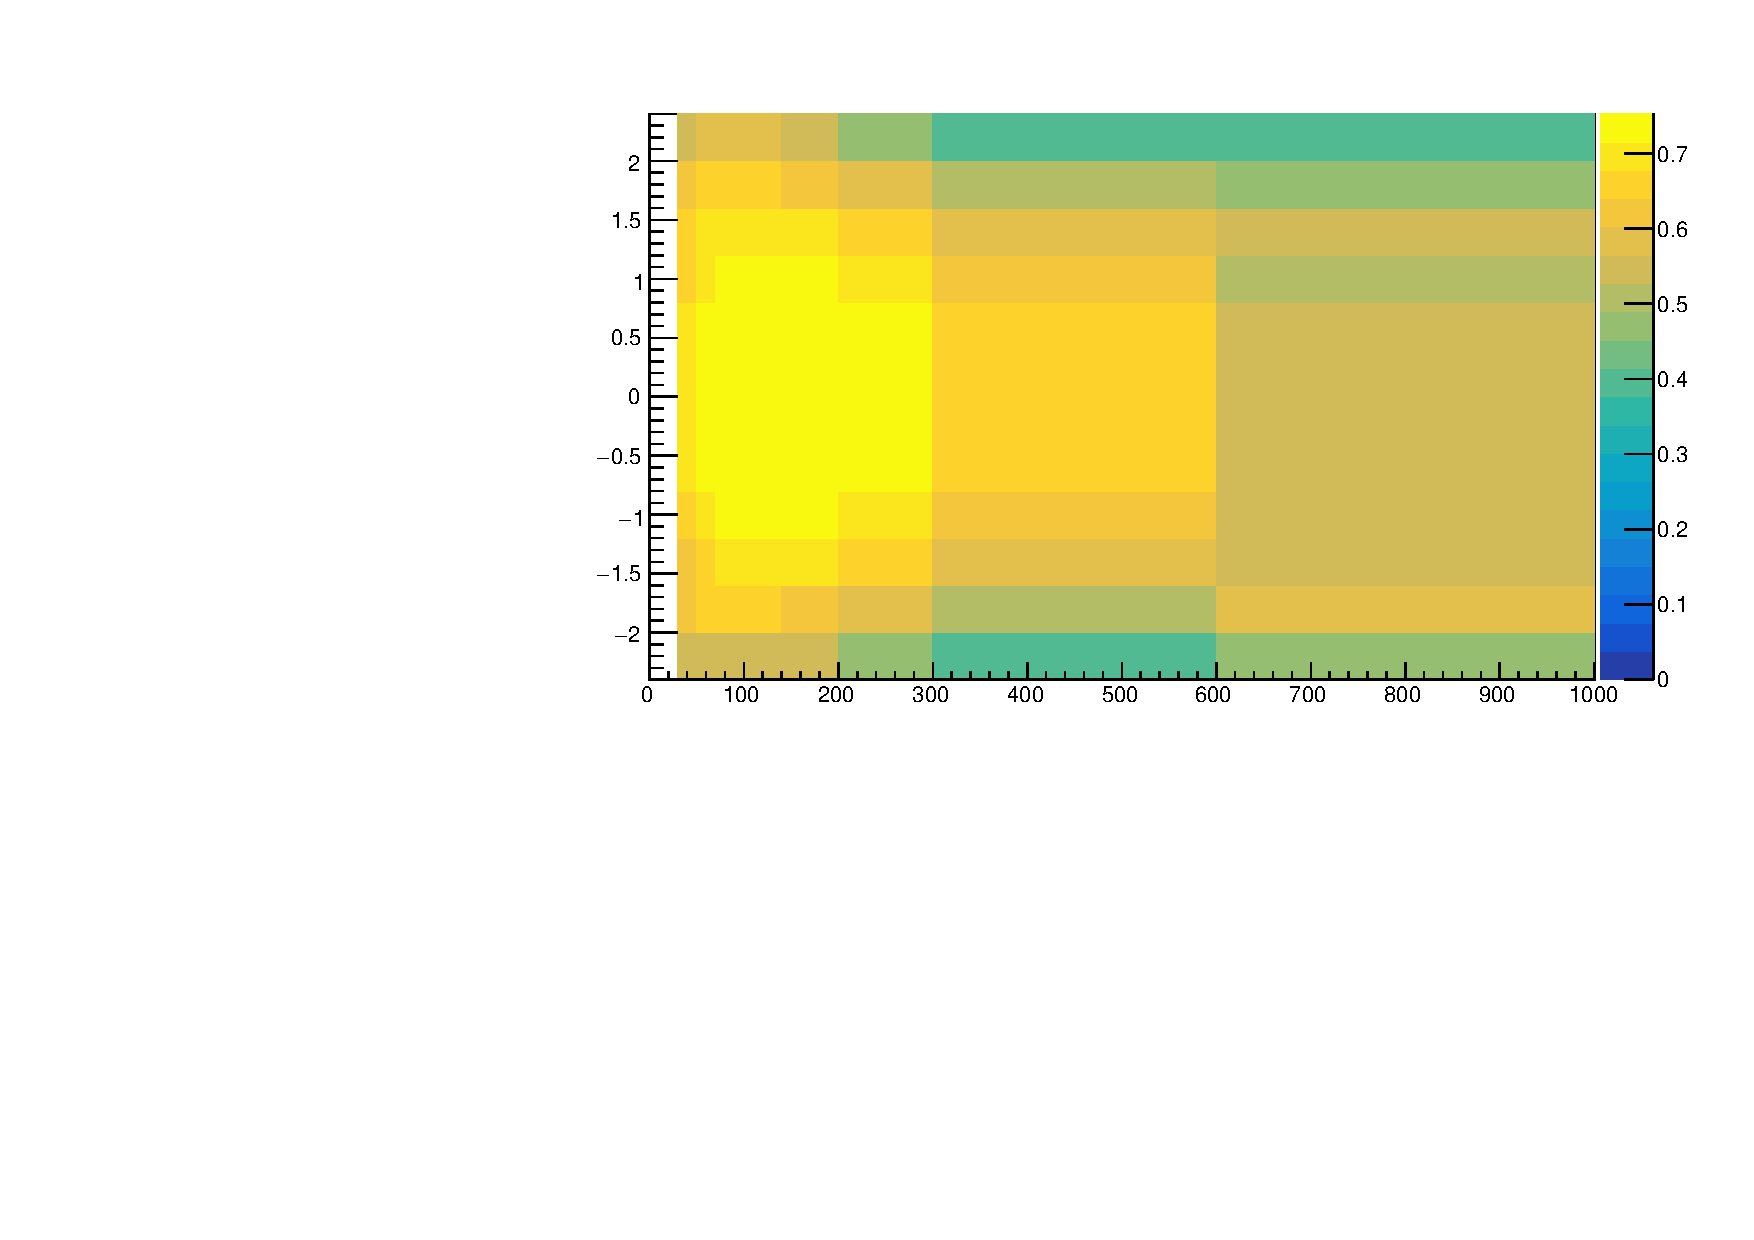
\includegraphics[width=0.45\textwidth]{Figures/DataMC/tt_eff_b.pdf}}
			    \subfigure[c]{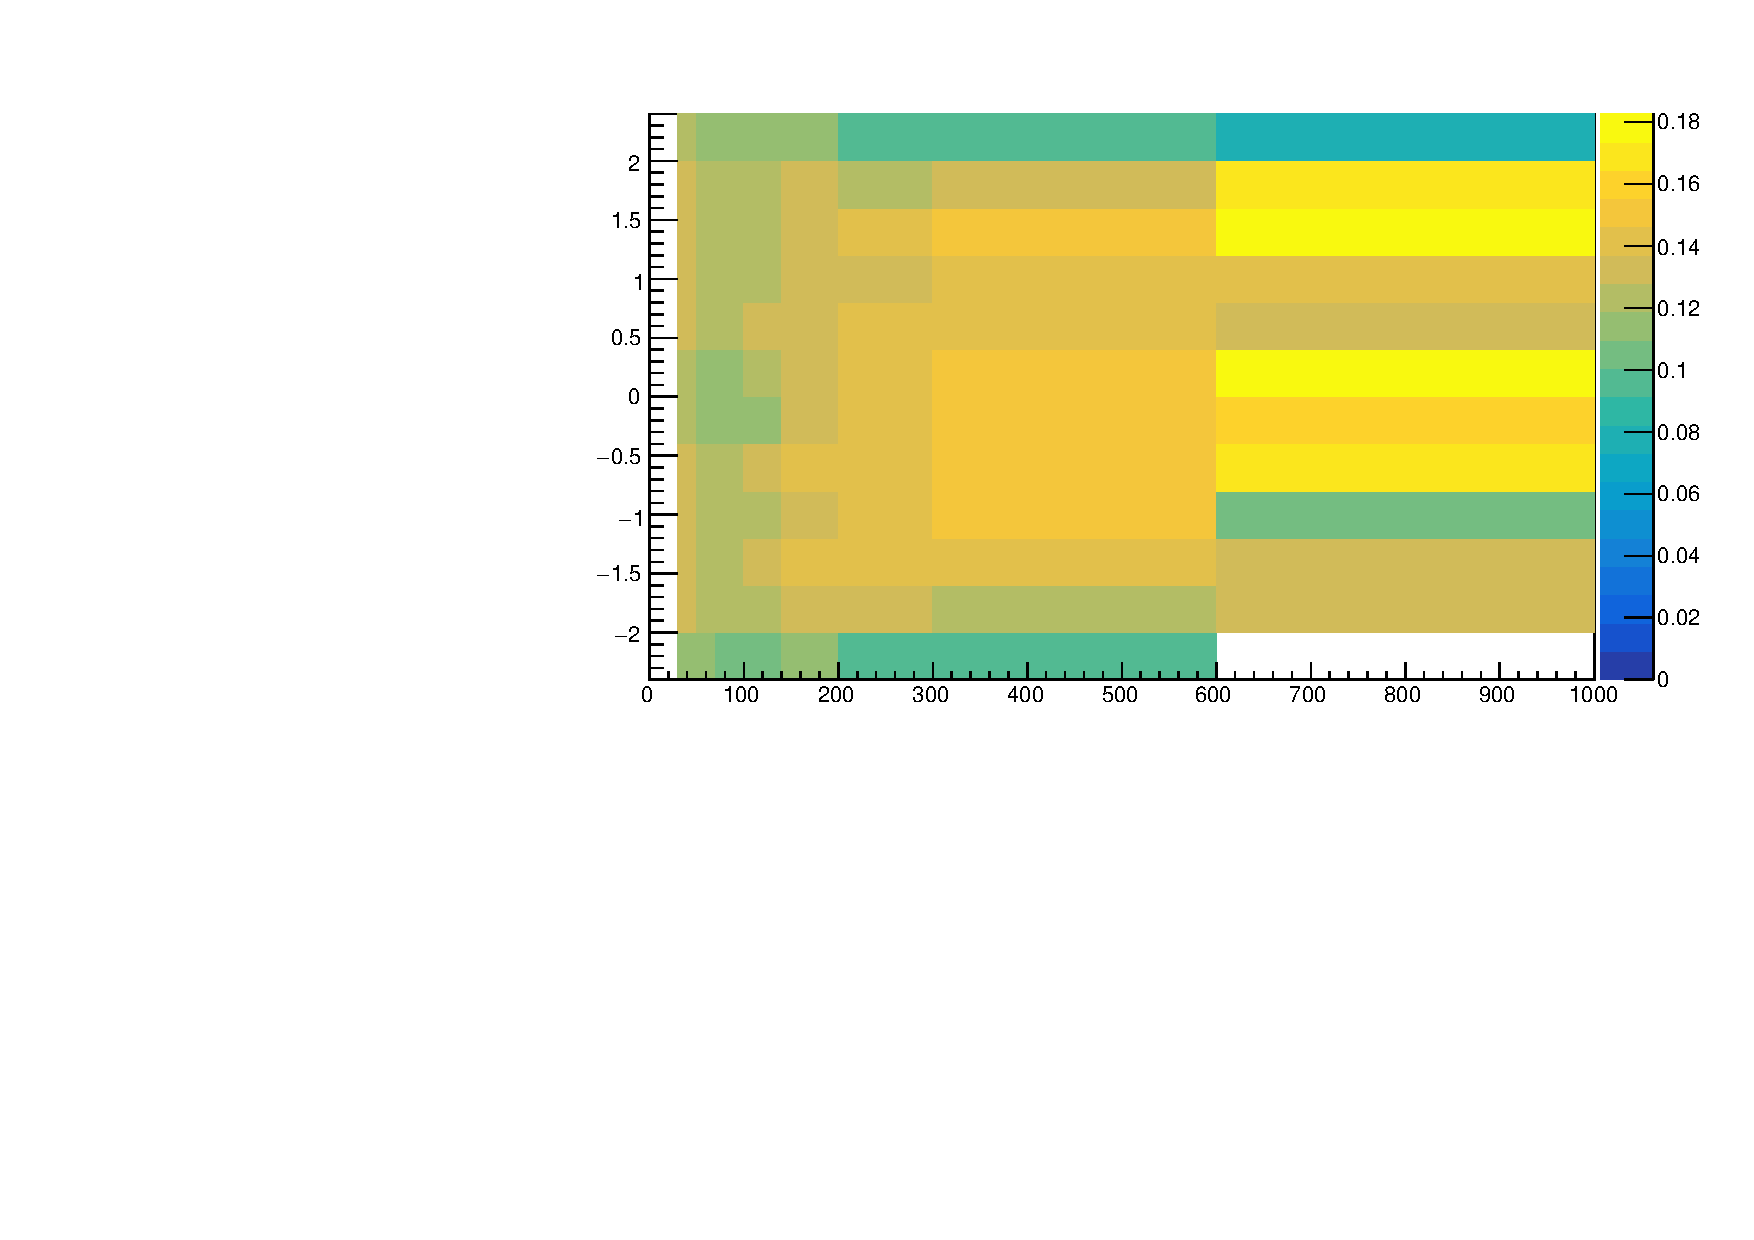
\includegraphics[width=0.45\textwidth]{Figures/DataMC/tt_eff_c.pdf}}\\
			    \subfigure[light(u,d,s,g)]{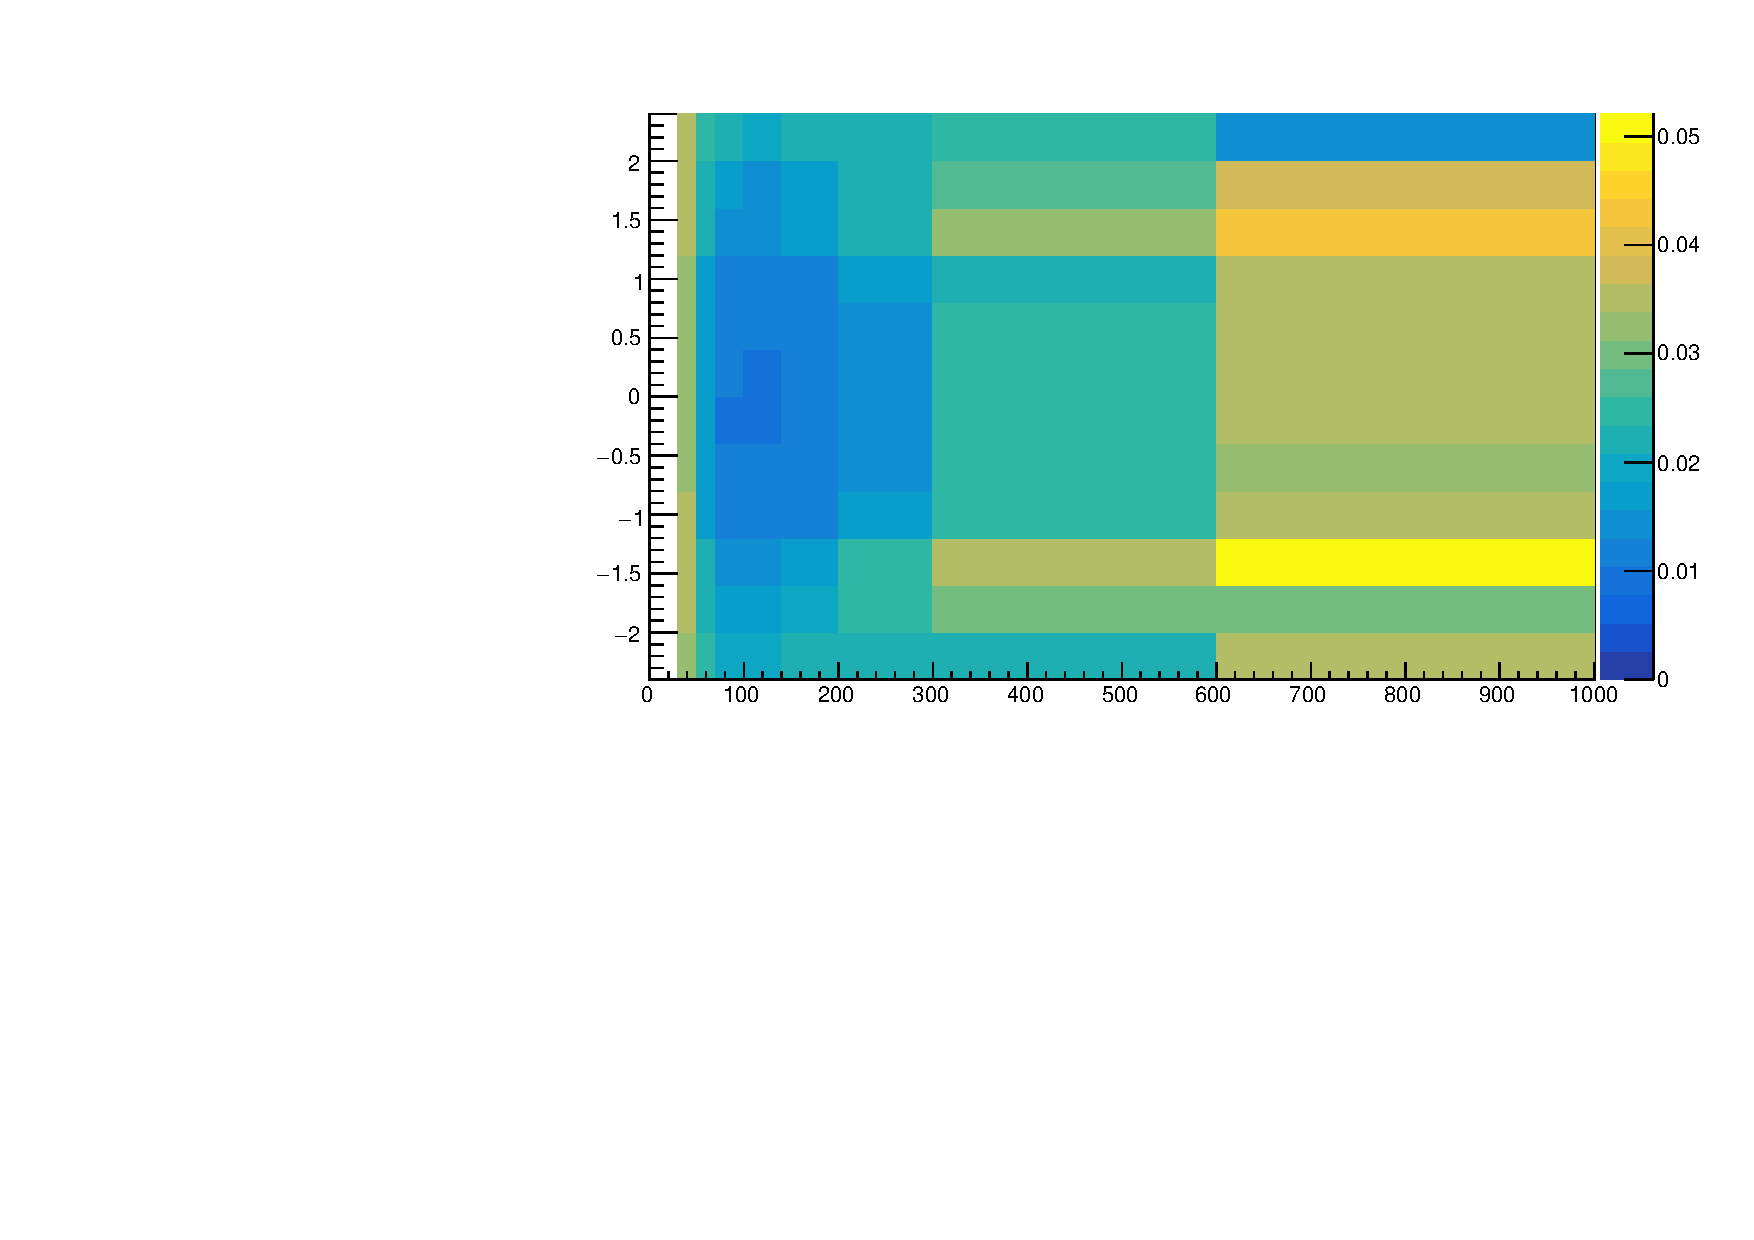
\includegraphics[width=0.45\textwidth]{Figures/DataMC/tt_eff_l.pdf}}
			   \caption{b-tagging efficiency of b, c, and light(udsg) flavor (x-axis:$p_T$, y-axis:$\eta$), under b-tagging working point Medium calculated by $t\bar{t}$ MC}
			\label{DataMC:fig:tt_eff_btag}
			\end{figure}
			\FloatBarrier

		\subsubsection{Weigh to Luminosity}
		\label{sssec:DataAndMC_lumi}

			The generated samples are generated under their individual cross section and generated events number. If we want to use these sample in analysis and act like the real data, they should be fixed to under same luminosity as data. Therefore, the weight to luminosity must be multiplied on any generated samples' events by Eq.\ref{eq:lumi_weight} with data luminosity 35.9$fb^{-1}$, samples' cross section, k factor, and generated events number from Table.\ref{DataMC:tb:process}.

			\begin{equation}
			w_{sample} = \frac{ L_{data} \cdot (\sigma_{sample} \cdot k)}{N_{sample,gen}}
			\label{eq:lumi_weight}
			\end{equation}



%%%--- TODO ---%%%



\FloatBarrier
